\newcommand{\sfact}{\mathcal{L}} %scaling factor
\newcommand{\speed}{\mathcal{S}} %speed function

\section{Introduction}
In this exposition to Adaptive MCMC I largely follow the review by \cite{Rosenthal2011}. I will discuss adaptivity for special cases of Metropolis-Hastings, as this is the case which has received the most attention in the literature. Tuning parameters of the sampling algorithm in MCMC, before the rise of adaptive MCMC, had to be done manually. This involves running the sampling algorithm several times and checking its performance. For an applied problem this performance check could be average loss with respect to a pre-specified loss function. Another possibility would be to try to get low Monte Carlo variance, an estimate of which is available in black box problems, i.e. problems in which the ground truth is unknown (the only case where one would apply MCMC anyway). Simply lowering Monte Carlo variance of course holds the danger of increasing the algorithms bias without noticing. We will discuss this in section \ref{sec:criteria_mcmc}.
As we will see in section \ref{sec:mcmc_scaling} though, in the MH-case one can also resort to tuning the algorithm for a certain acceptance rate. The theoretical results proving the optimality of an acceptance rate for a particular algorithm typically make strong assumptions regarding the target distribution $\targd$. However if these assumptions are violated, these acceptance rates still often times give good results experimentally.

A natural research direction then is to develop algorithms that adapt automatically to the target by using the information from collected samples. This way, one could hope to get rid of the time-consuming manual tuning. A natural first step in this direction is to adapt algorithm parameters in order to hit optimal acceptance rates. Another would be to adapt the proposal distribution to the posterior in some way.

\subsection{Criteria for evaluating MCMC algorithms}
\label{sec:criteria_mcmc}
In this section, I will focus on evaluation criteria that only make use of the output of the Markov Chain (as opposed to using criteria such as average loss on a dataset). First, we can compare the \emph{speed of convergence} of the Markov Chain. A Markov Kernel $\MK_1$ is said to converge faster than $\MK_2$ if
%$$sup \StateSp {\MK_1(x,A) , (A)}$$
$$sup_{A\subset \StateSp} |\MK^n_1(x,A)-\targd(A)| \leq sup_{A\subset \StateSp} |\MK^n_2(x,A)-\targd(A)| $$
\todo{Check: can I really use "markov kernel" here instead of "markov chain" as in Rosenthal? Is the total variation distance correct? shouldn't it be $A\in F$ where $F$ is the Sigma-Algebra on the statspace $\StateSp$?}
for any number of applications of the kernels $n$ and any $x$. Here $sup_{A\subset \StateSp} |\cdot - \cdot|$ is the total variation distance between two distributions, $\targd$ is the target density as usual and $\StateSp$ is the state space of the chain. The total variation distance is closely related to the Kullback-Leibler distance $D_\textrm{KL}$ in that $D_\textrm{KL}$ provides a tight upper bound via Pinsker's inequality  \citep[see Lemma 2.5 in][]{Tsybakov2008}.\\
Given some integrand $\targfunc$, $\MK_1$ has \emph{lower variance} than $\MK_2$ if
$$\Var(\sum_{i=1}^n \targfunc(\smp^{\MK_1}_i)/n) \leq \Var(\sum_{i=1}^n \targfunc(\smp^{\MK_2}_i)/n)$$
where $\smp^{\MK_j}_i$ is a sample from $\MK_j$. This of course depends on what integrand $\targfunc$ is to be computed, on the number of samples $n$ and on the starting state of the chains.\\
If $\MK$ leaves $\targd$ invariant (i.e. the Markov Kernel is ergodic or stationary wrt $\targd$), then for large $n$ we have $\Var(\sum_{i=1}^n \targfunc(\smp^{\MK}_i)/n) \approx n^{-1}\Var_\targd(\targfunc) \tau_{\targfunc}^\MK$ where 
$$\tau_{\targfunc}^\MK = \sum_{k=-\infty}^\infty \Corr(\targfunc(\smp^\MK_0),\targfunc(\smp^\MK_k)) = 1+2 \sum_{i=1}^\infty \Corr(\targfunc(\smp^\MK_0),\targfunc(\smp^\MK_i))$$ is the integral of the autocorrelation time under $\MK$ \todo{if this is an integral, why is there no division by something? Check Rosenthal in Handbook of MCMC again}. In other words, if there is no autocorrelation, we are left with the variance of $\targfunc$ under $\targd$, which is very intuitive - if our kernel really generates independent samples, it does not add any further variance to the estimate of $\Var_\targd(\targfunc)$. This results in another evaluation criterion: $\MK_1$ has \emph{smaller asymptotic variance} than $\MK_2$ if $\tau_{\targfunc}^{\MK_1} < \tau_{\targfunc}^{\MK_2}$.\\
Finally, a Kernel is better if the resulting chain takes larger steps in the state space on average. We say $\MK_1$ \emph{mixes faster} than $\MK_2$ if
$$ \Expect\{(\smp^{\MK_1}_k - \smp^{\MK_1}_{k-1})^2\} > \Expect\{(\smp^{\MK_2}_k - \smp^{\MK_2}_{k-1})^2\}$$
Here we can use the estimate $\Expect\{(\smp^{\MK}_k - \smp^{\MK}_{k-1})^2\} \approx n^{-1} \sum_{i=1}^n (\smp^{\MK}_i - \smp^{\MK}_{i-1})^2 $ where the samples are assumed to come from a chain that has converged. This expectation provides another insight into the performance of a Markov kernel. If in a Metropolis-Hastings setting a move is rejected, then $(\smp^{\MK}_i - \smp^{\MK}_{i-1})^2 = 0$. But a proposal perturbing the Chains state just a tiny bit and resulting in almost every move being accepted does not help much either because $(\smp^{\MK}_i - \smp^{\MK}_{i-1})^2$ will still be very small.\\
These criteria for evaluation Markov Kernels can be shown to be equivalent under certain conditions, resulting in the possibility to choose algorithm parameters in an optimal way if the conditions are met. If they are not met of course, different criteria might result in different decisions on how to set parameters.


\section{Scaling}
\label{sec:mcmc_scaling}
In MH, the optimal proposal distribution $\propd(\cdot|\smp')$ would be the target $\targd(\cdot)$, as in this case every move is accepted and we directly sample from the distribution of interest (the algorithm reduces to ordinary Monte Carlo). The case of MH used very often in practice however is that of a Random Walk using increments, i.e. a proposal is found by adding some increment $Z \sim \propd_\textrm{inc}(\sigma)$ to the current chain state, where $\scale$ is a scaling parameter of the density $\propd_\textrm{inc}$. The question now is which $\scale$ optimizes MCMC for generating samples that are as close to independent samples from the target $\targd$ as possible. A hint at the difference that different values of $\scale$ make might be drawn from a trace of a chains state space across samples. Figure \ref{fig:acc_rates_high_low_opt} shows the location of a chain with scalar state across samples, where  $\scale$ is the variance of normally distributed increments. When picking $\scale$ too low (upper right), almost every proposed move is accepted but the increments are tiny and the chain does not explore the state space well. On the other hand, when picking $\scale$ too high (upper right), proposals are only rarely accepted. Again, the exploration properties of the chain are poor.\\
When picking $\scale$ approximately optimal however (lower left), random walk sampling, informally, produces a trace closest to i.i.d. samples from the true target (lower right). In this case, proposals are neither mostly rejected nor mostly accepted. This insight initiated research into finding optimal acceptance rates for random walk and other MCMC algorithms.\\
While the theoretical results make rather strong assumptions as we will see, the optimal rates derived often give good results in practice even if assumptions are not met \cite{Rosenthal2011}.

\begin{figure}[htbp]
\begin{center}
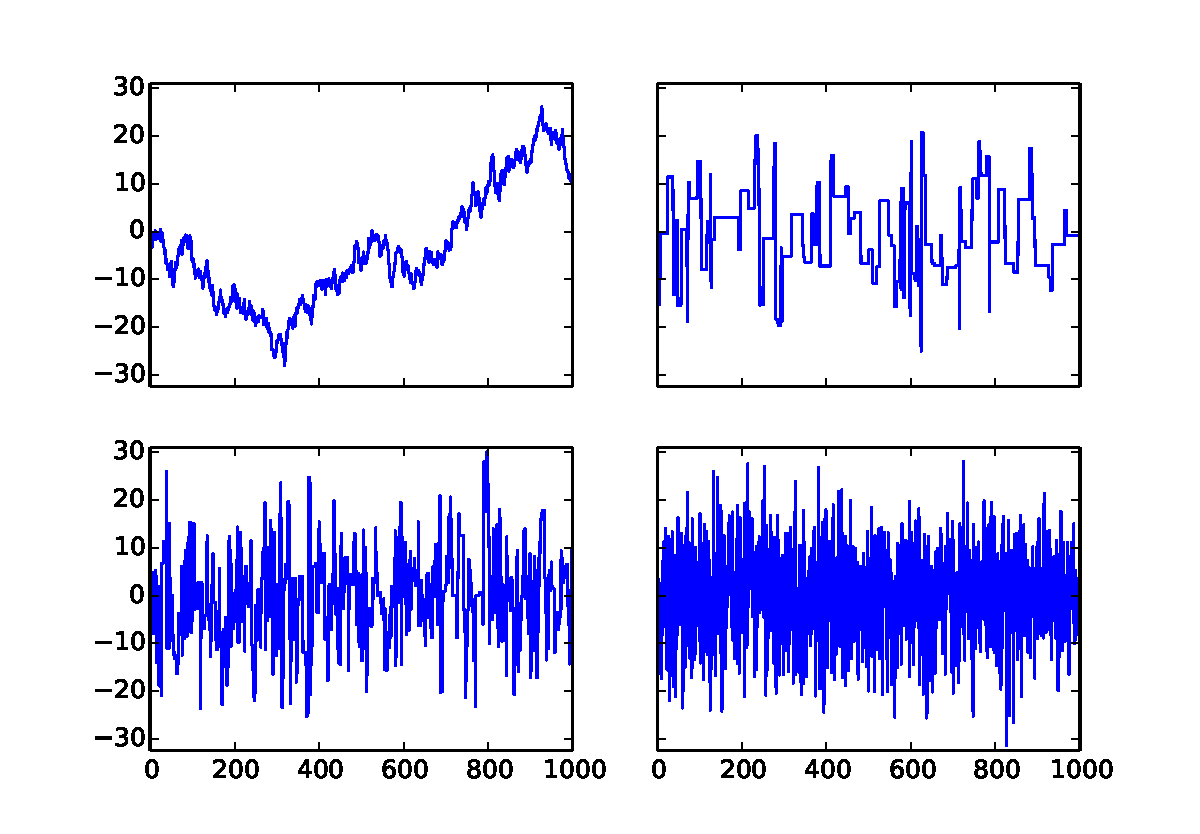
\includegraphics[width=\textwidth]{Figures/Acceptance_rates_high_low_optimal_iid.pdf}
\caption{\emph{Top}: Too high high (left, $0.96$) and too low (right, $0.13$) acceptance rates. \\\emph{Bottom}: approx. optimal rate for 1D target (left, $0.47$), i.i.d. target samples (right).}
\label{fig:acc_rates_high_low_opt}
\end{center}
\end{figure}

\subsection{Optimal scaling in Random Walk MH}
We consider $d$-dimensional target densities which are completely determined by the marginals, i.e. every component follows some density $\targd_c$ and is i.i.d.:
\begin{equation}
\label{eq:factortarget}
\targd(x_1, x_2, \dots, x_d) = \targd_c(x_1)\targd_c(x_2)\cdots\targd_c(x_d)
\end{equation}
A further assumption is that $\targd_c$ is smooth. Under these strong assumptions and for an increment distribution with isotropic covariance matrix $\DNorm(0,\scale^2I_d)$, \cite{Roberts1997} proved that the optimal acceptance rate is  exactly $0.234$ as $d \rightarrow \infty$. The derivation of the result proceeds along the following lines. Let $\scale = \sfact/\sqrt{d}$ where $\sfact> 0$. \cmt{FOLLOWING COPIED VERBATIM FROM ROSENTHAL -  Consult \cite{Roberts1997} for understanding!} \todo{Then as
$d \rightarrow \infty$, if time is speeded up by a factor of $d$, and space is shrunk by a factor of $\sqrt{d}$, then each component of the Markov chain converges to a diffusion having stationary distribution $\targd_c$, and speed function given by $\speed(\sfact) = 2\sfact^2\DNormCDF(-0.5\sqrt{I}\sf	act)$. Here $\DNormCDF$ is the CDF of the standard normal distribution, and $I$ is a constant given by $I = \Expect_{\targd_c}\left[  \left(\frac{\targd'_c(X)}{\targd_c(X)} \right)^2 \right] $}. Then by maximizing speed, the diffusion is optimal by all of the criteria given in \ref{sec:criteria_mcmc}:
$$\sfact_\textrm{opt} = \textrm{arg~max}_\sfact \speed(\sfact)$$
Nummerically, \cite{Roberts1997} found $\sfact_\textrm{opt} = 2.38/\sqrt{I}$ \todo{did \cite{Roberts1997} really state that? check!}, and as they also derived the asymptotic acceptance rate as $2\DNormCDF(-0.5\sqrt{I}\sfact)$, we can just plug in $\sfact_\textrm{opt}$ to get the optimal acceptance rate $A_\textrm{opt}$ (again, under the strong assumptions above and asymptotically for $d \rightarrow \infty$) as  $$A_\textrm{opt} = 2\DNormCDF(-0.5\sqrt{I}~\sfact_\textrm{opt}) = 0.234$$.
\todo{More results for more general cases, all leading to about $A_{opt} =0.234$ with some exceptions}

\subsection{Optimal scaling in MALA}
The Metropolis Adjusted Langevin Algorithm (MALA) \cite{Roberts1996} is similar to random walk MH with the difference that the random increments to the state of the Markov Chain are not centered on $0$. Rather, the increments at a given current state $\smp_n$ are distributed as $\DNorm(\frac{\scale^2}{2}\nabla \textrm{log}~\targd(\smp_n),\scale^2I_d)$ (see \ref{sec:lmc} for an overview of MALA and its truncated variant MALTA). In this case, \cite{Roberts1998} proved that under the assumption \eqref{eq:factortarget} and $\scale = \sfact/\sqrt[6]{d}$, we get 
 $$A^\textrm{MALA}_\textrm{opt} =  0.574$$
 The optimal scaling $\scale$ is bigger than in the random walk case \todo{check in original \cite{Roberts1996}}. 
 \begin{figure}[htbp]
\begin{center}
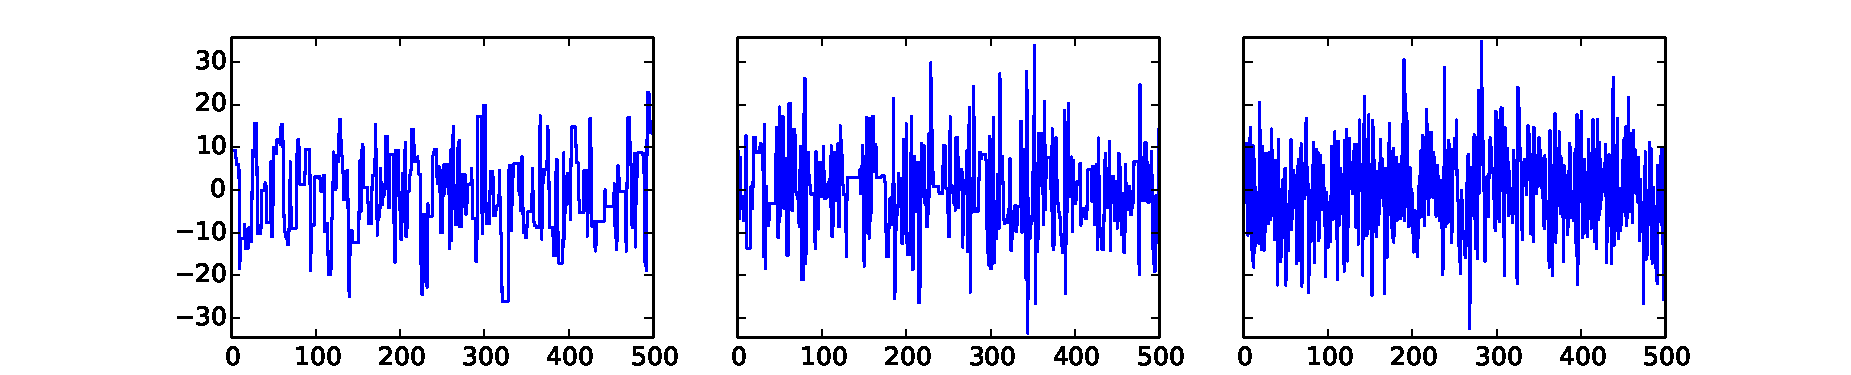
\includegraphics[width=\textwidth]{Figures/RW_vs_MALA_vs_iid.pdf}
\caption{Traces of state space of RW ($0.43$ left) and MALA ($0.58$ middle) with chains tuned for optimal acceptance rate, i.i.d. samples (right) for comparison}
\label{fig:rw_vs_mala}
\end{center}
\end{figure}

\subsection{Adaptivity}
When optimal acceptance rates are known, the experimenter might just run the MCMC algorithm and tune $\scale$ to get close to $A_\textrm{opt}$. This of course is tedious as it requires human intervention. While this can be automated in a straight forward way, tuning a single scale parameter might not be the only type of adaptivity that makes sense. The following section will thus look at the general case of algorithms that aim at automatically improving the sampling procedure while still ensuring ergodicity with respect to the target density.

\section{Automatic adaptation and ergodicity of sampling algorithms}
In the following, we will take a closer look at \emph{adaptive MCMC} algorithms and under which conditions they are ergodic with respect to some target density. Traditional Markov Chain Monte Carlo algorithms assume that the transition from state $\smp_n$ to state $\smp_{n+1}$ is markovian (i.e. can be described by a Markov Kernel $\MK(\cdot, \smp_n)$, hence \emph{Markov Chain}). Confusingly, adaptive MCMC algorithms do not necessarily construct a Markov Chain with respect to $\smp$. For many algorithms, the process $\{\smp_n,\MK_n\}_{n=0}^\infty$ (where $\MK_n$ is the kernel used at iteration $n$) is Markovian, but not even this is a necessary condition. A more appropriate name would thus be something along the lines of \emph{adaptive ergodic Monte Carlo}.\\
In the following, we use a set of Markov Kernels $\{\MK_i\}_{i \in \mathcal{I}}$, all of which have $\targd$ as their unique stationary distribution. At the $n$th iteration, we denote by $\MK_n$ the Kernel that is used to generate a new sample. One might expect that, as every $\MK_i$ has $\targd$ as stationary distribution, any mixture of the kernels in $\{\MK_i\}_{i \in \mathcal{I}}$ has the same property. However, \cite{Rosenthal2011} provides a simple counter example. Let $f$ be a probability mass function that is nonzero for each element of $\StateSp=\{1,2,3,4\}$

\begin{center}
\begin{tabular}{c|c c c c}
$x$ & $1$ & $2$ & $3$ & $4$\\
\hline 
$\targd(x)$ & $0.333$ & $0.001$ & $0.333$ & $0.333$
\end{tabular}
\end{center}

and $\targd(x) = 0$ for $x \notin \StateSp$. Now let $\MK'$ be a Metropolis-Hastings kernel with proposal $\propd(\cdot | \smp_n) = \textrm{Uniform}\{ \smp_n -1,  \smp_n+1\}$ and $\MK''$ one with proposal $\propd(\cdot | \smp_n) = \textrm{Uniform}\{\smp_n -2, \smp_n -1,  \smp_n+1, \smp_n +2\}$. Then because of the MH correction, both $\MK'$ and $\MK''$ are reversible and thus ergodic with respect to $\targd$. Now consider the following algorithm for adaptivity: set $\MK_{n+1} = \MK''$ if the $n$th move was accepted, $\MK_{n+1} = \MK'$ else. Now the adaptive algorithm can get stuck with using $\MK'$ in the state $\smp=1$ for many consecutive proposals and only has a probability of $0.001/0.333$ to switch to the usage of $\MK''$. Thus, informally, the adaptive mixture of ergodic (wrt $\targd$) kernels results in a sampling procedure that will yield state $1$ way more often than the equally probable states $3,4$.

Thus, we need to establish sufficient conditions for ensuring that adaptive MCMC algorithms preserve ergodicity. To this end, \cite{Roberts2007} provided results for a broad class of algorithms under rather weak assumptions. If the assumptions hold, asymptotic convergence (in the number of samples) of the sample approximation to the target $\targd$ holds, i.e.
\begin{equation}
\lim_{n \rightarrow \infty} \sup_{A\subseteq \StateSp} \|P(\smp_n \in A) - \targd(A)\| = 0
\end{equation}
 and furthermore a weak law of large numbers, i.e.
 \begin{equation}
\lim_{n \rightarrow \infty} \sum_{i=1}^n \targfunc(\smp_i) = \targd(\targfunc)
\end{equation}
for all bounded integrands $\targfunc: \StateSp \rightarrow \mathbb{R}$. The assumptions are  \emph{Diminishing Adaptation}
\begin{equation}
\label{eq:dimin_adapt}
\lim_{n \rightarrow \infty} \sup_{x \in \StateSp} \|\MK_{n+1}(x, \cdot) - \MK_{n}(x, \cdot)\| = 0 \textrm{ in probability}
\end{equation} 
and \emph{Bounded Convergence} (or \emph{Containment})
\begin{equation}
\label{eq:bound_conv}
\{M_\epsilon(\smp_n, n)\}_{n=0}^\infty \textrm{ is bounded in probability}
\end{equation} 
where $M_\epsilon(x, n) = \inf\{\|\MK_n^i(x, \cdot) - \targd(\cdot) \| \leq \epsilon : i \geq 1 \}$ for some $\epsilon > 0$ is called the $\epsilon$ convergence time for kernel $\MK_n$ when starting from state $x$. Assumption \eqref{eq:dimin_adapt} is the stronger of the two. In English, it says that the amount of adaptation goes to $0$ for growing $n$. An important note here is that there can still be an infinite total amount of adaptation (as the assumption is not  $\sum_{n=1}^\infty \sup_{x \in \StateSp} \|\MK_{n+1}(x, \cdot) - \MK_{n}(x, \cdot)\|< \infty$). Also, the limit $ \lim_{n \rightarrow \infty} \MK_n$ does not need to exist, i.e. the sequence of used Markov Kernels does not have to converge to some fixed kernel. One way of ensuring \eqref{eq:dimin_adapt} is to adapt at iteration $n$ with some probability $p(n)$ and have $\lim_{n \rightarrow \infty} p(n) = 0$. Also, in the case where $\MK_n$ uses an average of the previous $n$ samples, then as the new sample only contributes $\frac{1}{n}$th to the average, the amount of adaptation goes to $0$ for growing $n$.\\
Assumption \eqref{eq:bound_conv} on the other hand holds when $\StateSp \times S_\MK$ is finite (where $S_\MK$ is the set of used Markov Kernels), or compact in a topology where the kernels in $S_\MK$ or the Metropolis-Hastings proposal densities $\{\propd_n\}_{n=1}^\infty$ have a jointly continuous density \citep{Rosenthal2011,Roberts2007}. It basically says that for any combination of current sample $\smp$ and chosen kernel $\MK$, iteratively applying $\MK$ will ensure that the sampling approximation is less than $\epsilon$ away from target $\targd$ in a finite number of iterations. Thus, this condition is often easily satisfied \citep[though counterexamples can be constructed, see ][]{Rosenthal2011}.\\
In the following I will introduce some of the adaptive MCMC algorithms from the literature. The first important modern algorithm is the Adaptive Metropolis algorithm of \cite{Haario2001}.

\subsection{Adaptive Metropolis}
The first representative algorithm in the class of adaptive MCMC, the Adaptive Metropolis (AM) Algorithm \cite{Haario2001}, fits a Gaussian approximation with mean $\bar{\smp}_{n}$ and covariance matrix $C_n$ to the samples acquired up until iteration $n$. This is achieved by the recursion formula
\begin{equation}
\label{eq:haario_cov}
C_n = \begin{cases}
C_0 & n \leq n_0 \\
\scale_d (cov(X_0,\dots, X_{n-1}) + \epsilon I)& n > n_0
\end{cases}
\end{equation}
For an initial $C_0$ and some $n_0$ and where $\scale_d>0$ and $\epsilon>0$ are tunable parameters. Adding $\epsilon$ to the diagonal ensures that $C_n$ does not degenerate to zero. To update $C_n$ with a new sample $X_n$, we can use a recursion formula 
\begin{equation*}
C_{n+1} = \frac{n-1}{n} C_n + \frac{\scale_d}{n} \left (n\bar{X}_{n-1}\bar{X}^T_{n-1} - (n+1) \bar{X}_{n}\bar{X}^T_{n} + {X}_{n}{X}^T_{n}  + \epsilon I\right )
\end{equation*}
The proposal distribution for a new point given the last sample is $\smp_n$ then is
\begin{equation}
\label{eq:am_prop_orig}
q_\textrm{AM}(\cdot|\smp_n) = \DNorm(\smp_n, C_n)
\end{equation}
and a value $\smp^*$ is accepted with probability $min(1,\targd(\smp^*)/\targd(\smp_n))$. \cite{Haario2001} suggested that $\scale_d$ will be set depending only on the dimensionality of the domain of $\targd$. In the case where $\targd$ can be approximated by a gaussian, \cite{Rosenthal2011}  suggest to use $\scale_d = 2.38^2/d$. A minor variant of the AM algorithm is given in \cite{Roberts2009}. Instead of adding $\epsilon$ to the diagonal, they propose using a mixture proposal
\begin{equation}
\label{eq:am_prop_mod}
q'_\textrm{AM}(\cdot|\smp_n)  = (1-\beta)\DNorm(\smp_n, \scale_d~cov(X_0,\dots, X_{n-1}) ) + \beta \DNorm(\smp_n, \Sigma)
\end{equation}
 for a $\beta \in (0,1)$ and some fixed covariance matrix $\Sigma$.
 
 Since the adaptation at the $n$th step decreases as $\BigO(\frac{1}{n})$, the diminishing adaptation assumption \eqref{eq:dimin_adapt} is satisfied. The bounded convergence conditon \eqref{eq:bound_conv} holds if the target density $\targd$ decays at least polynomially in each coordinate, thus ensuring that the entries of the fitted covariance matrix will stay finite and actually converge to some fixed value. In conclusion, AM is ergodic with respect to $\targd$. The literature \citep{Haario2001,Roberts2009} and my own experiments in section \ref{sec:eval} suggest that AM is a very robust algorithm even for very high dimensions and outperforms non-adaptive sampling algorithms using gradient information such as Hamiltonian Monte Carlo \citep{Neal2011} tuned for optimal acceptance rate. The main problem AM poses is a computational one. In high dimensions, computing a matrix inverse or Cholesky factorization of the empirical covariance matrix after one new sample is acquired is prohibitively slow. One way to ameliorate this problem is to only adapt every $k$ iterations (and take all $k$ new samples into account). Another is to directly update the empirical covariance in its Cholesky form \citep[see e.g. ][]{Rasmussen2006}. In this case, the proposal in \eqref{eq:am_prop_mod} is the natural choice, as it is not  clear whether rank one updates are possible if some $\epsilon$ is added to the diagonal of the empirical covariance. However, updating the eigendecomposition of the empirical covariance one might still be able to use of the proposal distribution \eqref{eq:am_prop_orig}\footnote{Personal communication with Yee Whye Teh}.

\subsection{Adaptive MALTA}
An algorithm similar to AM making use of gradient information is the adaptive Metropolis Adjusted Langevin Algorithm with truncated drift \citep[adapt. MALTA, ][]{Atchade2006}. It uses parameters $0 < \epsilon_1 <A_1, \epsilon_2 >0$ and $\gamma_n$ which depends on the iteration index. To the process $(\smp_n)$ on the sample space $\StateSp$ adaptive MALTA adds an adaptation process $(\mu_n, \Gamma_n, \scale_n)$ on a space denoted $\Theta$. To give an intuition, $\mu_n$ will be (close to) a fit of the empirical mean of $(\smp_n)$, $\Gamma_n$ will be close to the empirical covariance of $(\smp_n)$ and the parameter $\scale_n$ is a scale parameter, similar to the parameter of the same name in AM. Let $C_n = \scale^2_n(\Gamma_n+\epsilon_2 I)$ for some parameter $\epsilon_2$. When the last sample is $\smp_n$, adaptive MALTA uses a proposal distribution
$$\propd(\cdot| \smp_n) = \DNorm(\smp_{n} + \frac{C_n}{2} D(n, \smp_{n}), C_n)$$
and a proposed move to $\smp^*$ is accepted with the standard MH probability
$$p_n^\textrm{acc}(\smp^*|\smp_n) = \textrm{min}\left(1, \frac{\targd(\smp^*)q(\smp_n|\smp^*)}{\targd(\smp_n)q(\smp^*|\smp_n)} \right)$$
The subscript $n$ hints at the fact that the acceptance probability depends on the parameter values at time $n$ through $\propd$.
 $D(\cdot, \cdot)$ is a drift function and \cite{Atchade2006} suggests
$$D(k, x) = \frac{\delta}{\textrm{max}(\delta, |\nabla~\textrm{log}~\targd(x)|)}\nabla~\textrm{log}~\targd(x)|$$
The scale parameter is constrained to the interval $[\epsilon_1,A_1]$ by the projection
\begin{equation*}
p_1(\scale) = 
\begin{cases}
\epsilon_1 & \scale <\epsilon_1 \\
A_1 & \scale > A_1 \\
\scale & \textrm{else}
 \end{cases}
 \end{equation*}
The covariance $\Gamma_n$ is constrained to lie in the convex compact cone defined by the projection
\begin{equation*}
p_2(\Gamma) = \begin{cases}\Gamma &|\Gamma| \leq A_1 \\ 
 \frac{A_1}{|\Gamma|}\Gamma &\textrm{else}
 \end{cases}
 \end{equation*}
where $|\cdot|$ is the Frobenius norm. Finally, $\mu_n$ is constrained to the ball $B(0,A_1)$ in $\mathbb{R}^d$ (where $d$ is the dimensionality of the problem) by the projection
\begin{equation*}
p_3(\mu) = \begin{cases}A_1 &|\mu| \leq A_1 \\ 
 \mu &\textrm{else}
 \end{cases}
 \end{equation*}
 Suppose we have generated a new sample $\smp_{n+1}$. Now the parameters are adapted using the following equations.
\begin{eqnarray*}
\mu_{n+1} &= &p_3(\mu_n+\gamma_n(\smp_{n+1} -\mu_n))\\
\Gamma_{n+1} &=& p_2(\Gamma_n + \gamma_n((\smp_{n+1}-\mu_n)(\smp_{n+1}-\mu_n)^T-\Gamma_n)\\
\scale_{n+1} &= &p_1(\scale_n+\gamma_n(p_n^\textrm{acc}(\smp^*|\smp_n)-\tau))
\end{eqnarray*}
Where $\tau$ is the optimal acceptance rate that the algorithm should try to attain and $\gamma_n$ is a factor decreasing the amount of adaptation for each new sample. Concretely,  $\lim_{n \rightarrow \infty}\gamma_n = 0$ and \cite{Atchade2006} used $\gamma_n = 10/n$. The values for the other parameters where set as $\epsilon_1 = 10^{-7}, \epsilon_2 = 10^{-6}, A_1=10^7$. 

As is evident even from this concise exposition to adaptive MALTA, it is a complex algorithm with many parameters (even though according to \cite{Atchade2006} the algorithm is not very sensitive to $\epsilon_1,\epsilon_2$ and $A_1$, so they might be considered fixed). Of course it has the advantage of working correctly even if the expectation or variance of $\targd$ does not exist. However, even when tuned to optimal acceptance rates, I found the performance of adaptive MALTA to often be worse than that of AM.


